
\section{Dataset and archive details}\label{app:data}
UCI consumer indices are 5, 37, 70, 103, 136, 168, 201, 234, 267 and 300 in the public
LSTNet-format electricity matrix. Alabama plant indices are 3, 21, 39, 57, 75, 93, 111
and 130. Main observed traces use the initial 8,000 raw observations, except the two
minute-level ETT channels (12,000) and ERCOT channels (16,000). The ETT columns are
ETTh1/OT, ETTh2/OT, ETTm1/HUFL and ETTm2/OT.

The two cross-consumer splices concatenate 1,500-point segments starting at raw offset
1,000 from clients (10,40,70,100) and (25,90,140,210). Seasonal constructions use clients
20 and 80, concatenating 1,200-point windows starting at offsets 4392, 8784, 13128 and
17544. They deliberately omit the intervening chronology. Synthetic series have length
6,000, seeds 1 and 7, AR coefficient 0.7, a sinusoid of period 200 and four piecewise
mean/innovation-scale regimes $(0,1),(0,2.2),(5,0.8),(-3,1.6)$.

The multi-horizon panel uses electricity clients 20 and 80, solar plants 10 and 30,
ETTh1/OT, the first cross-consumer splice, seasonal client 20 and synthetic seed 1.
Origins stop 24 steps before the raw-series end for every horizon, ensuring the same
origins within that panel. Public data sources are the LSTNet data repository\footnote{\url{https://github.com/laiguokun/multivariate-time-series-data}},
ETDataset\footnote{\url{https://github.com/zhouhaoyi/ETDataset}}, ERCOT historical
load\footnote{\url{https://www.ercot.com/gridinfo/load/load_hist}} and GEFCom2014.


\clearpage
\section{Detailed delayed-feedback results}
\begin{table}[h!]\centering\small
\caption{Multi-horizon comparison. Gains use the residual--ACI score at the same horizon.
Local error is in percentage points. Tuning never uses test labels.}
\label{tab:horizon}\begin{tabular}{lrrr}
\toprule
Horizon / method & Gain (\%) & Cov. (\%) & Local (pp) \\
\midrule
1 / residual/aci & 0.00 & 89.99 & 1.77 \\
1 / native-scale/aci & 12.91 & 90.01 & 1.31 \\
1 / cqr/aci & 14.35 & 90.03 & 1.39 \\
1 / cqr/pi-log & 14.94 & 90.02 & 1.50 \\
1 / cqr/saocp & 12.48 & 90.69 & 2.10 \\
1 / cqr/faci & 15.42 & 89.61 & 1.68 \\
1 / cqr/aci/tuned & 14.87 & 90.09 & 1.97 \\
6 / residual/aci & 0.00 & 89.46 & 2.44 \\
6 / native-scale/aci & -11.77 & 89.64 & 1.96 \\
6 / cqr/aci & 13.89 & 89.54 & 2.06 \\
6 / cqr/pi-log & 16.21 & 90.00 & 2.53 \\
6 / cqr/saocp & 5.26 & 84.09 & 6.13 \\
6 / cqr/faci & 15.50 & 86.74 & 3.81 \\
6 / cqr/aci/tuned & 15.47 & 89.74 & 3.13 \\
24 / residual/aci & 0.00 & 87.10 & 4.90 \\
24 / native-scale/aci & -52.27 & 87.32 & 4.50 \\
24 / cqr/aci & 13.15 & 87.34 & 4.52 \\
24 / cqr/pi-log & 17.09 & 89.96 & 4.86 \\
24 / cqr/saocp & 6.56 & 79.98 & 10.16 \\
24 / cqr/faci & 15.57 & 82.72 & 7.94 \\
24 / cqr/aci/tuned & 11.62 & 88.09 & 5.46 \\
\bottomrule
\end{tabular}
\end{table}


\clearpage
\section{Per-series primary comparison}
\begin{table}[h!]\centering\small
\caption{Default CQR--ACI compared with default residual--ACI, averaged over four backbones.}
\begin{tabular}{lrr}
\toprule
Series & Gain (\%) & Coverage (\%) \\
\midrule
ETTh1\_OT & 3.12 & 89.98 \\
ETTh2\_OT & 8.27 & 89.99 \\
ETTm1\_HUFL & 8.74 & 89.99 \\
ETTm2\_OT & 3.70 & 89.97 \\
electricity\_c103 & 5.21 & 89.97 \\
electricity\_c136 & 4.87 & 89.99 \\
electricity\_c168 & 5.90 & 89.93 \\
electricity\_c201 & 5.33 & 89.96 \\
electricity\_c234 & 6.61 & 90.00 \\
electricity\_c267 & 4.74 & 90.01 \\
electricity\_c300 & 17.21 & 89.91 \\
electricity\_c37 & 8.05 & 89.97 \\
electricity\_c5 & 8.43 & 89.95 \\
electricity\_c70 & 5.72 & 89.89 \\
ercot\_COAST & 0.77 & 90.01 \\
ercot\_ERCOT & -1.53 & 90.00 \\
ercot\_NORTH & 1.86 & 89.97 \\
seasonal\_elec\_c20 & 6.25 & 90.09 \\
seasonal\_elec\_c80 & 10.90 & 90.00 \\
solar\_p111 & 34.92 & 89.90 \\
solar\_p130 & 34.37 & 89.92 \\
solar\_p21 & 36.12 & 89.97 \\
solar\_p3 & 35.42 & 89.97 \\
solar\_p39 & 35.01 & 90.07 \\
solar\_p57 & 35.63 & 89.94 \\
solar\_p75 & 36.33 & 89.98 \\
solar\_p93 & 34.21 & 89.97 \\
spliced\_electricity\_4seg & 11.36 & 90.10 \\
spliced\_electricity\_4seg\_b & 13.27 & 90.02 \\
synthetic\_T6000 & 0.31 & 89.99 \\
synthetic\_T6000\_s7 & -0.42 & 90.02 \\
\bottomrule
\end{tabular}
\end{table}


\clearpage
\section{Confirmation controller diagnostics}\label{app:confirmation}
\begin{table}[htbp]\centering\scriptsize
\caption{Confirmation contrasts at $h=24$. Each row contains four series and two models.
Gain and median are paired interval-score improvements (\%); A is the first method in
the comparison and B the second. Coverage is in percent, target 90\%. Correlated pairs
are retained without interpreting the win count as independent replications.}
\label{tab:confirmation}\begin{tabular}{llrrrrr}
\toprule
Comparison & Family & Gain & Median & Wins & Cov. A & Cov. B \\
\midrule
Native / residual, COP & FX & 11.10 & 2.73 & 7/8 & 89.76 & 89.72 \\
Native / residual, COP & Traffic & 33.22 & 31.79 & 8/8 & 90.45 & 91.40 \\
Native / residual, issued ACI & FX & 3.79 & 1.06 & 8/8 & 89.03 & 89.10 \\
Native / residual, issued ACI & Traffic & 13.20 & 11.92 & 8/8 & 89.83 & 90.20 \\
Issued / shared, CQR & FX & 8.62 & 5.01 & 8/8 & 89.03 & 86.12 \\
Issued / shared, CQR & Traffic & 8.24 & 7.98 & 8/8 & 89.83 & 89.63 \\
\bottomrule
\end{tabular}

\end{table}

\begin{table}[h!]\centering\scriptsize
\caption{Unified comparison on the revisited panel at $h=24$. IS ratio averages
per-pair interval scores divided by that pair's residual rolling-quantile score;
lower is better. Family coverage is percent (target 90\%). Local is the family-balanced
150-origin absolute coverage error in percentage points; Singleton is percent.
Original rows retain locked-grid results, wide ACI and multi-step PID are subsequent
sensitivities. PI-log and SF-OGD retain fixed defaults, not tuned optima.}
\begin{tabular}{llrrrrr}
\toprule
Score & Controller & IS ratio & FX cov. & Traffic cov. & Local & Singleton \\
\midrule
Residual & Rolling & 1.000 & 87.48 & 89.58 & 6.77 & 0.000 \\
Residual & Shared, original & 1.063 & 87.75 & 88.51 & 5.66 & 0.000 \\
Residual & Issued, original & 0.929 & 89.10 & 90.20 & 6.58 & 0.000 \\
Residual & Shared, wide & 1.066 & 87.57 & 88.07 & 6.14 & 0.000 \\
Residual & Issued, wide & 0.939 & 88.53 & 89.72 & 6.57 & 0.000 \\
Residual & PI-log & 2.341 & 89.92 & 90.03 & 6.36 & 2.873 \\
Residual & SF-OGD & 5.146 & 90.18 & 90.03 & 6.63 & 4.356 \\
Residual & COP & 1.177 & 89.72 & 91.40 & 6.39 & 0.249 \\
Residual & Grouped ACI & 0.984 & 86.76 & 89.23 & 5.74 & 0.000 \\
Residual & Fixed-scale OGD & 1.096 & 86.11 & 90.50 & 7.14 & 0.344 \\
Residual & Implicit-delay & 1.057 & 86.05 & 90.03 & 6.98 & 0.000 \\
CQR & Rolling & 0.852 & 87.78 & 89.41 & 6.37 & 0.038 \\
CQR & Shared, original & 0.937 & 86.12 & 89.63 & 5.79 & 0.167 \\
CQR & Issued, original & 0.853 & 89.03 & 89.83 & 6.12 & 0.025 \\
CQR & Shared, wide & 0.860 & 88.02 & 89.53 & 6.21 & 0.031 \\
CQR & Issued, wide & 0.851 & 88.14 & 89.88 & 6.22 & 0.044 \\
CQR & PI-log & 2.048 & 90.04 & 89.98 & 6.06 & 3.011 \\
CQR & SF-OGD & 4.528 & 90.17 & 90.09 & 6.47 & 4.377 \\
CQR & COP & 0.879 & 89.76 & 90.45 & 5.57 & 0.028 \\
CQR & Grouped ACI & 0.904 & 87.45 & 89.67 & 5.62 & 0.018 \\
CQR & Fixed-scale OGD & 0.884 & 88.25 & 90.92 & 6.13 & 0.126 \\
CQR & Implicit-delay & 0.884 & 88.33 & 90.92 & 6.07 & 0.069 \\
Signed error & Multi-step PI & 1.163 & 86.89 & 89.22 & 6.68 & 0.024 \\
Signed error & Multi-step PID & 1.176 & 86.85 & 89.21 & 6.92 & 0.065 \\
\bottomrule
\end{tabular}

\end{table}


\clearpage
\section{Algorithm and integrity checks}\label{app:integrity}
The primary evidence concerns the archived forecasts, not a reranking of freshly
downloaded checkpoints. Offline spot checks reproduce the point and five quantile outputs
exactly at 21 selected origins per model across three main-panel series, for 84 checked
model--origin cases. For the two Chronos models, matching the original default batch
grouping of 256 contexts resolves differences observed with a seven-context batch.
TimesFM's checked outputs match the local 2.0 checkpoint through its Hugging Face adapter;
Moirai matches after its original quantile-rearrangement step. Current checkpoint hashes
and environment versions are recorded. These checks support archive provenance but
do not constitute a rerun of every forecast, and original checkpoint commits were not
stored with every archive. Possible pretraining exposure to
public benchmark data also precludes an assertion that all test series were unseen during
pretraining.


The executable checks test future-target perturbations at lags 1, 6 and 24, identical
evaluation masks, unit rescaling, exact stored-level selection, empirical quantile
agreement, interval-score arithmetic, finite behavior under zero-width forecasts and
the reference SAOCP expert recursion. Data validation independently reconstructs target
values from local raw-series loaders. Cache records include archive, protocol and code
hashes; aggregations reject stale code/protocol outputs.

Source implementations and licenses are retained for SAOCP/FACI and PID. The SAOCP
numerical check covers its nonnegative-score expert recursion, without validating a
theorem for signed or delayed extensions. \ref{app:rules} specifies controller
conventions; the artifact retains complete grids, failures and tail misses. Recorded
runtimes include possible compilation overhead and do not measure neural inference speed.

Additional checks cover clipping identities, COP source-recursion equivalence,
target/issue-time conversion, grouped feedback assignment and implicit proximal
optimality against an independent optimizer and subgradient conditions. Protocols
and exploratory amendments remain separately identifiable.

The asymmetric multi-step PID comparison matches the unmodified author implementation
over 24 horizons and four configured scorecasters, including future-target perturbations.
Check records and tolerances accompany the artifact. The later full AcMCP-CSS
weather comparison has 96 complete-trajectory checks and 60 independent scorecast refits.


\section{Matched implicit-update ablation}\label{app:implicit}
The implicit ablation exactly solves the proximal objective already considered by
\citet{hu2026cop}. With $p=1-\alpha$, pinball loss $\ell_p(u)=u(p-\ind\{u<0\})$,
and a fixed prefix-scaled step $\eta=\gamma(\max_{i<600}s_i-\min_{i<600}s_i)$
(range floored at $10^{-12}$), it uses
\begin{equation}\label{eq:prox}
 b_t=b_{t-1}+\eta(e_{t-h}-\alpha),\qquad
 q_t=\arg\min_q\left\{\frac{(q-b_t)^2}{2}
       +h\eta\,\widehat{\mathbb E}_t[\ell_p(S-q)]\right\}.
\end{equation}
The same 300-score convention supplies the empirical distribution. The matched OGD
ablation sets $q_t=b_t$. Both select from $\{0.005,0.02,0.05,0.1\}$ and these values
divided by $h$. The point of this control is to distinguish an implicit correction's
incremental value from the fixed scale and learning rate. The development screen also
retains half-step and explicit corrections; it did not validate a new algorithm.

The delay-scaled implicit correction in Equation~\eqref{eq:prox} has a plausible
stationary rationale. If the true and proxy CDFs have local densities $g>0$ and
$\widehat g\geq0$, its deterministic linearized delayed gain is
$c=\eta g/(1+h\eta\widehat g)$. With a correct slope it is below $1/h$ and hence
inside the classical shared-state stability boundary in Equation~\eqref{eq:stability}.
For fixed slopes, however, this is simply a smaller effective gain. It predicts no
automatic advantage over suitably tuned basic gradient updating, and the argument
does not cover changing empirical distributions or atoms.

The development screen evaluates 3,200 configuration instances, retaining every
setting. At $h=24$, implicit-delay CQR improves interval score by 2.54\% over issued
ACI and 2.08\% over delay-tuned COP, but only 0.23\% over matched fixed-scale OGD.
It fails the locally recorded continuation criterion of at least 3\% against both
strong baselines, even before further validation. On the subsequent confirmation
panel, its matched-OGD gain is $-0.08\%$: $-0.30\%$ for exchange rates and $0.14\%$
for traffic, with seven of 16 positive differences. We therefore retain this result
as a negative ablation, not a new main method. A more sophisticated update formula
is insufficient evidence of additional predictive information or better adaptation.



\section{Rate, delay and clipping diagnostics}\label{app:rates}
Figure~\ref{fig:ratesurface} uses the common ten-rate subset of the wide grid to
display the rate--delay sensitivity. It shows every listed rate's test behavior,
not a test-based selector. The original selected shared-state CQR score at each
horizon is a common per-pair denominator for both structures. The additional
delay-scaled rates also participate in selection and remain in the full result files.

\begin{figure}[htbp]\centering
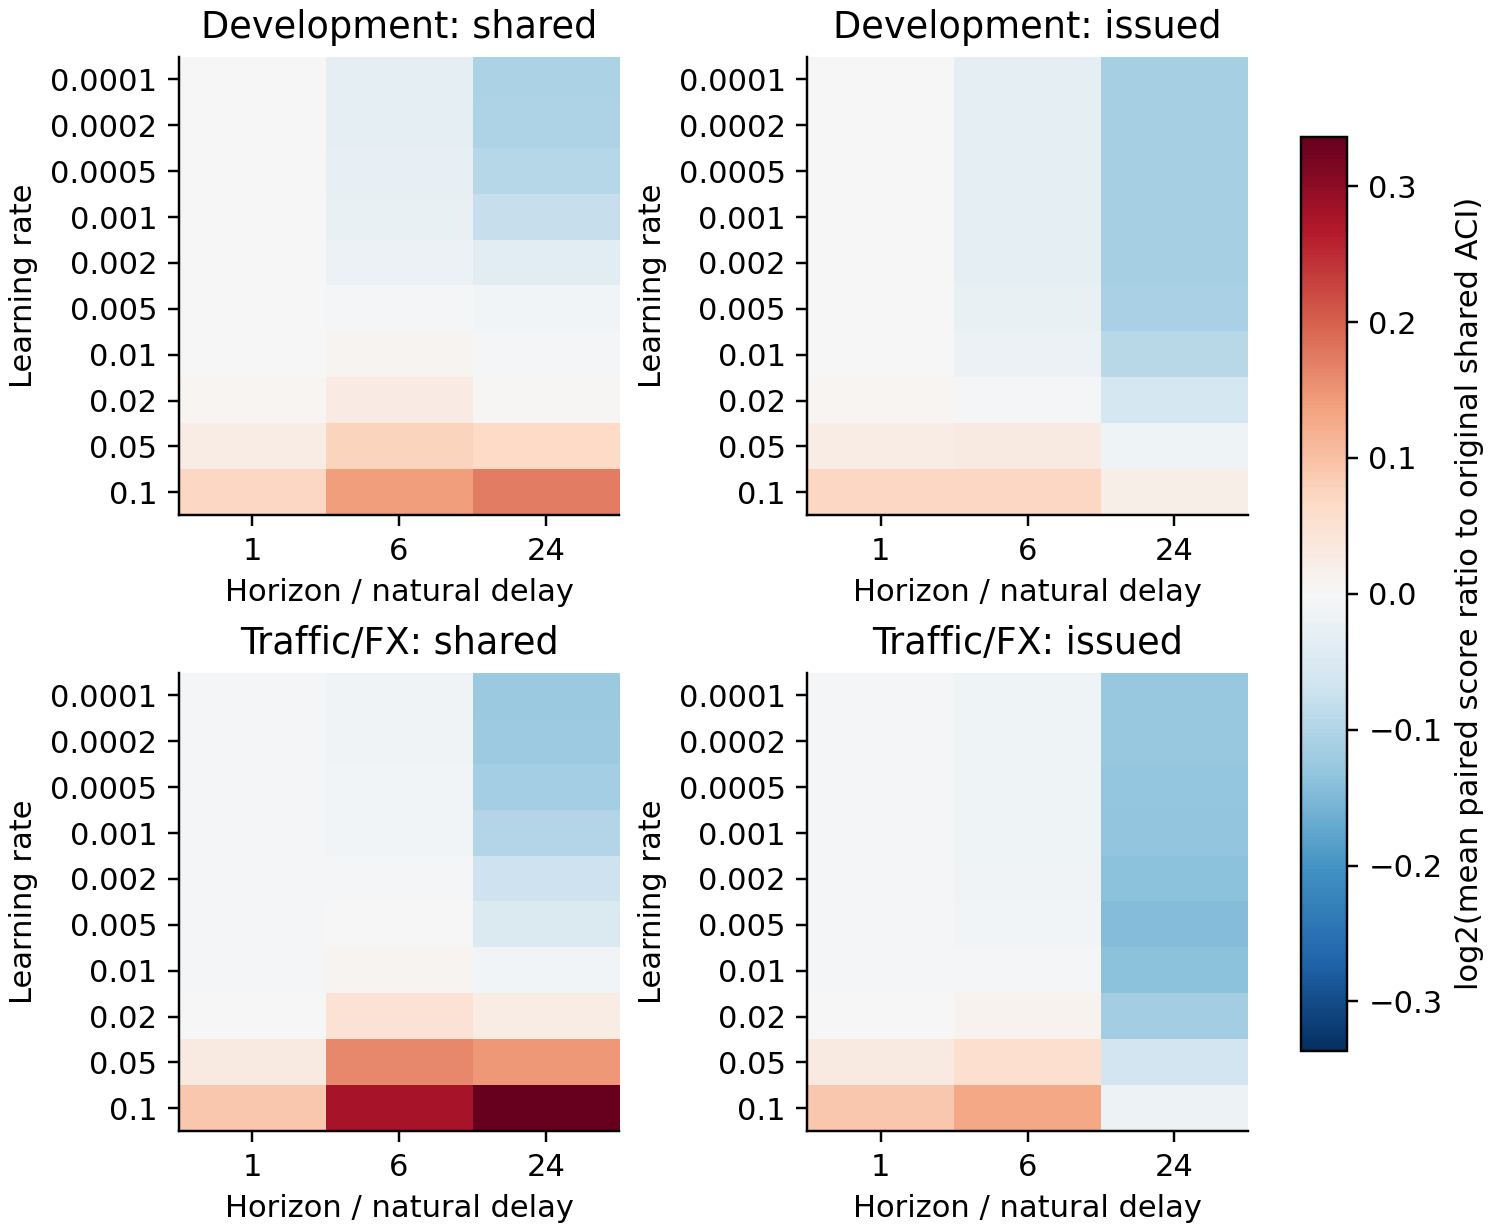
\includegraphics[width=\textwidth]{figures/rate_delay_surface.png}
\caption{CQR rate--delay surfaces. Color is the base-two logarithm of the mean
paired interval-score ratio to original-grid shared CQR; zero means equal score.
Positive values are worse. Development and revisited panels have 16 pairs each.
Validation selects configurations; the plotted test surface is descriptive.}
\label{fig:ratesurface}\end{figure}

\begin{table}[htbp]\centering\scriptsize
\caption{Exact revealed-test miscoverage decomposition, CQR, $h=24$, in percentage
points. Clip plus Endpoint equals Excess up to rounding. Each interval was issued
in the test segment and revealed by the last archive origin. The last 24 issued
test intervals are pending; their separately recorded contribution bounds the
difference from full issued-test coverage by $24/N_{\rm test}$.}
\begin{tabular}{lllrrr}
\toprule
Panel & Grid & State & Clip & Endpoint & Excess \\
\midrule
Development & original & shared & 1.801 & 0.004 & 1.804 \\
Development & original & issued & 0.023 & 0.393 & 0.415 \\
Development & scaled & shared & 0.043 & 0.398 & 0.441 \\
Development & scaled & issued & 0.023 & 0.611 & 0.633 \\
Development & wide & shared & 0.043 & 0.487 & 0.530 \\
Development & wide & issued & 0.023 & 0.642 & 0.664 \\
Traffic/FX & original & shared & 2.117 & 0.033 & 2.150 \\
Traffic/FX & original & issued & 0.135 & 0.461 & 0.596 \\
Traffic/FX & scaled & shared & 0.336 & 0.681 & 1.017 \\
Traffic/FX & scaled & issued & 0.135 & 0.863 & 0.998 \\
Traffic/FX & wide & shared & 0.336 & 0.909 & 1.245 \\
Traffic/FX & wide & issued & 0.182 & 0.834 & 1.016 \\
\bottomrule
\end{tabular}

\end{table}

For the controlled simulations, the response is prescribed as
$M_t(a)=\clip\{0.1+g(a-a_t^*),0,1\}$, with $g\in\{1,4\}$ and $h\in\{1,6,24\}$.
Runs contain 12,000 steps. Stationary runs use effective gains at 0.5 and 1.2 times
the shared linear boundary. Tracking runs use $a_t^*=0.1,0.2,0.06$ in three
4,000-step segments and the original three rates plus their delay-scaled versions.
Deterministic response feedback and Bernoulli feedback are kept distinct, with
20 fixed seeds for the latter, yielding 1,764 controller runs. In the deterministic
$h=24,g=4,\gamma=0.005$ tracking example, mean absolute state error over the first
500 steps after both changes is 0.0198 for shared and 0.0978 for issued updating.
This is a specified-response illustration, not a forecast score or a causal diagnosis
of all empirical losses.

\begin{figure}[htbp]\centering
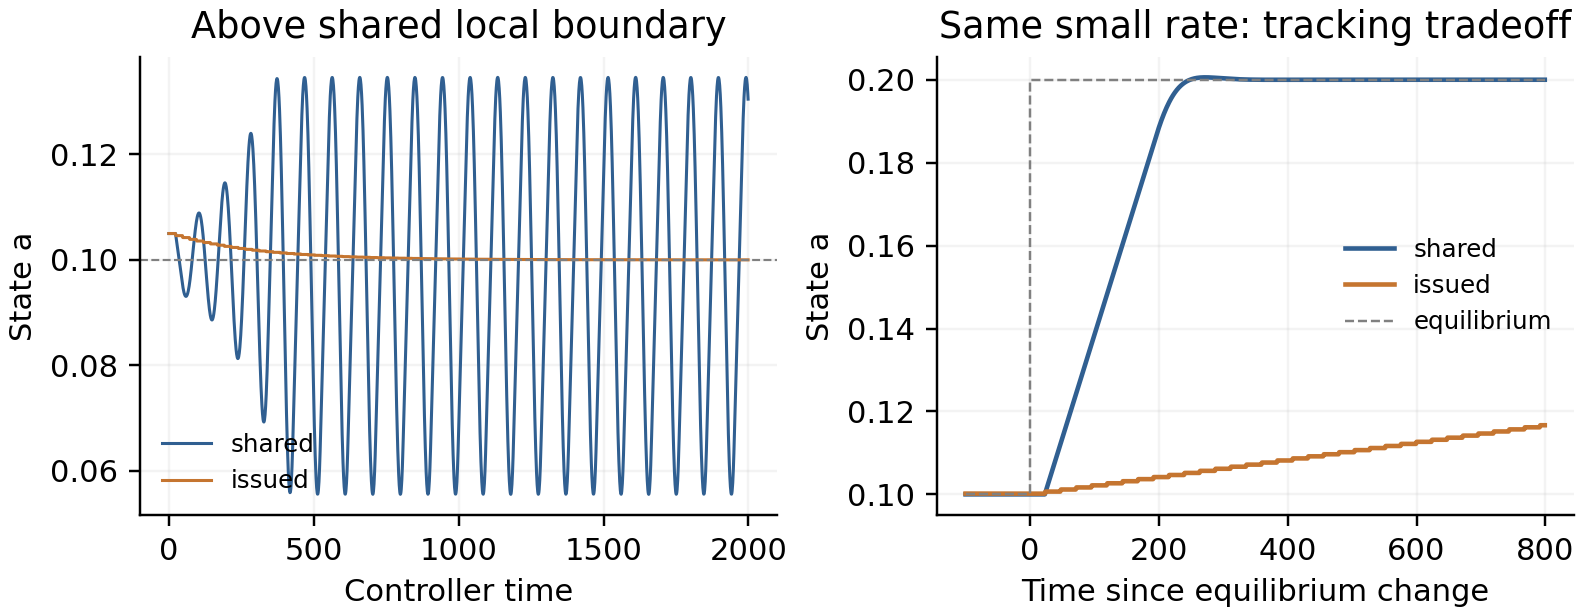
\includegraphics[width=\textwidth]{figures/controlled_dynamics.png}
\caption{Deterministic response illustrations at $h=24,g=4$. Left: effective gain
1.2 times the shared local boundary. Right: $\gamma=0.005$, below the boundary for
both states, following an equilibrium change. State clipping and response saturation
are explicit; the trajectories illustrate stability and tracking, not coverage guarantees.}
\label{fig:dynamics}\end{figure}


\section{Photovoltaic score components}\label{app:solarparts}
\begin{table}[htbp]\centering\small
\caption{One-step PV interval-score components, averaged over the original 32 pairs.
IS equals Width plus Lower plus Upper, where the last two are the $2/\alpha$-weighted
miss-distance penalties. These means use the shared PV data units; the headline
relative gains are instead calculated per pair before averaging. All outcome-defined
groups are evaluation-only.}
\begin{tabular}{lllrrrr}
\toprule
Settings & Score & Group & IS & Width & Lower & Upper \\
\midrule
default & cqr & all & 2.629 & 1.766 & 0.555 & 0.308 \\
default & cqr & positive & 5.978 & 3.831 & 1.386 & 0.761 \\
default & cqr & zero & 0.498 & 0.454 & 0.025 & 0.020 \\
default & residual & all & 4.046 & 2.284 & 1.218 & 0.544 \\
default & residual & positive & 7.607 & 3.086 & 3.126 & 1.395 \\
default & residual & zero & 1.781 & 1.773 & 0.006 & 0.002 \\
tuned & cqr & all & 2.575 & 1.816 & 0.476 & 0.282 \\
tuned & cqr & positive & 5.888 & 4.017 & 1.183 & 0.688 \\
tuned & cqr & zero & 0.467 & 0.417 & 0.027 & 0.023 \\
tuned & residual & all & 3.240 & 1.987 & 0.820 & 0.432 \\
tuned & residual & positive & 6.775 & 3.626 & 2.066 & 1.082 \\
tuned & residual & zero & 0.991 & 0.945 & 0.027 & 0.019 \\
\bottomrule
\end{tabular}

\end{table}
Each pair's all-observation score and coverage is reconstructed by weighting its
zero- and positive-output components by their own sample fractions. This check is
performed before any averaging across plants and models. There are no negative
targets in this evaluated PV panel. The original default and validation-tuned
overall scores are reproduced from the archived predictions before decomposition.


\section{Additional sensitivities}\label{app:sensitivity}
\subsection{Scale mismatch can amplify interval widths}
Normalization is helpful when the predicted scale tracks error size. It can also amplify
historical mistakes. For positive scales, a native-normalized residual interval has width
\begin{equation}\label{eq:ratio}
 2\tilde b_t\,Q_{1-a_t}\!\left(\{|y_i-m_i|/\tilde b_i:i\in\mathcal H_t\}\right).
\end{equation}
If more than the upper-tail fraction of the calibration history has error magnitude $c$
and scale $\varepsilon$, its empirical threshold can approach $c/\varepsilon$. A later
scale $B$ then produces width $2Bc/\varepsilon$. A relative floor keeps the expression
finite, but does not eliminate a large historical-to-current scale ratio. Additive CQR
does not have this particular multiplicative amplification mechanism, although it can
still perform poorly when the base endpoints or update rule are unsuitable.

This argument does not establish that every normalization loss is caused by exact zero
bands. Both scale transitions and very small but nonzero widths matter. We therefore
retain all failures, record floor activation and score extremes, and avoid a test-dependent
score cap. Nor does the argument establish that a proposed regularizer must improve
prediction: the validation and test experiments must decide that question.

\subsection{Normalization failures and unsuccessful selection}
At $h=24$, native-scale ACI has a mean gain of $-52.27\%$, despite a 12.91\% gain on
the same panel at $h=1$. Large losses occur on the Chronos-Bolt solar series and on
constructed scale switches, as well as smaller losses elsewhere. For example, its
interval-score increase on Chronos-Bolt/solar-p10 is 286.35\% relative to residual--ACI.
These cases are consistent with historical-to-current scale mismatch in
Equation~\eqref{eq:ratio}; exact zero bands are not required. The artifacts include
width-floor activation rates and normalized-score extremes for every trace.

Regularized normalized CQR does not reliably fix the problem. Across all three horizons,
its mean gains range from $-12.50\%$ at $\lambda=0$ to $-9.65\%$ at $\lambda=1$ for the
reported endpoint choices, compared with 13.80\% for additive CQR--ACI. The validation
selector increases the main-panel gain from 13.57\% to 13.72\%, but its multi-horizon
mean is 13.36\%, below fixed CQR--ACI. We retain this failed hypothesis instead of
expanding the selector grid on the test results. Prefix-based selection remains causal,
but a causal procedure need not transfer well across later regimes.

\subsection{Nominal levels, rearrangement and native-output provenance}
The primary CQR--ACI benefit persists at 80\% and 95\% calibrated targets
(Table~\ref{tab:sensitivity}). Omitting quantile rearrangement changes the primary mean
gain from 13.57\% to 13.56\%. The main conclusion is therefore not driven by sorting,
although sorting matters more for some individual normalized-score configurations.

\begin{table}[htbp]\centering\small
\caption{CQR--ACI sensitivity, using default residual--ACI at the same nominal level as
the denominator. Dense archives are a repeated-output sensitivity, not new independent data.}
\label{tab:sensitivity}\begin{tabular}{lrrr}
\toprule
Panel / miscoverage & Pairs & Gain (\%) & Cov. (\%) \\
\midrule
main-a0.2 & 124 & 9.85 & 80.01 \\
main-a0.1 & 124 & 13.57 & 89.98 \\
main-a0.05 & 124 & 14.00 & 94.90 \\
dense-a0.1 & 93 & 13.80 & 89.98 \\
gefcom-a0.1 & 39 & 19.63 & 89.99 \\
\bottomrule
\end{tabular}
\end{table}

The genuine stored 0.1--0.9 native bands achieve average main-panel coverage of 81.89\%
(Chronos-2), 87.04\% (Chronos-Bolt), 81.96\% (Moirai) and 77.57\% (TimesFM), against
their 80\% nominal mass. These values include both overcoverage and undercoverage.
They cannot substantiate a claim that all models' native 90\% intervals under-cover.

The dense archive requires additional care. TimesFM still stores only the five original
levels, so it supplies no genuine 0.05--0.95 comparison. Chronos-Bolt's stored 0.05 and
0.95 outputs equal its 0.1 and 0.9 outputs on approximately 99.86\% of rows after
rearrangement; requesting more levels did not create independent tail information.
Chronos-2's stored 0.05--0.95 band attains 91.69\% coverage at a nominal 90\%.
We therefore do not use the dense files to claim exact full-distribution CRPS or a
universal native 90\% calibration result.

\setlength{\bibsep}{4pt}


\section{Controller implementation details}\label{app:rules}
\subsection{One-step and delayed rule variants}
We compare seven rules using the same score streams and observation schedule.
\begin{enumerate}
\item \emph{Split}: a fixed empirical $(1-\alpha)$ quantile of the initial 600 scores.
\item \emph{Rolling}: an empirical $(1-\alpha)$ quantile of the latest $W=450$ revealed scores.
\item \emph{Clipped ACI}: replace $\alpha$ in the rolling quantile by $a_t$, updated as
\begin{equation}\label{eq:aciappendix}
 a_t=\clip_{[0.001,0.999]}\{a_{t-1}+\gamma(\alpha-e_{t-d})\},\qquad \gamma=0.02,
\end{equation}
where $e_i=\ind\{y_i\notin C_i\}$ and the update is applied only after an issued interval's
outcome becomes available. The equation suppresses idle steps before that event.
\item \emph{SF-OGD adaptation}: with $M=\max_{i<600}|s_i|$, update the threshold by
$q\leftarrow q-Mg/\sqrt{\sum g^2}$, where $g=\alpha-e$. We initialize at the prefix
quantile and allow signed thresholds. This coverage-gradient implementation is described
explicitly rather than claimed identical to every tie/projection convention in the
published wrapper \citep{bhatnagar2023saocp}.
\item \emph{PI-log adaptation}: a proportional threshold update and logarithmic tangent
integrator inspired by \citet{angelopoulos2023pid}. With $k$ revealed post-initialization
errors and $E_k=\sum_{j=1}^k(e_j-\alpha)$,
\begin{equation}\label{eq:pi}
 z_k=z_{k-1}+\gamma M(e_k-\alpha),\qquad
 q_k=z_k+M\tan\!\left(E_k\frac{\log(k+2)}{k+1}\right).
\end{equation}
The tangent saturates to signed infinity outside $(-\pi/2,\pi/2)$. The initial $z$ is the
prefix quantile. We use a fixed prefix scale, omit scorecasting and retain our causal
delay convention; this is not full reference PID.
\item \emph{SAOCP adaptation}: the strongly adaptive coin-betting expert update from
the author implementation \citep{bhatnagar2023saocp}, with default lifetime multiplier 8
and prefix scale $\sqrt{3}M$. The accelerated residual-score implementation agrees
numerically with an independent driver of the original expert class. For signed CQR we
remove its nonnegative projection; with delayed feedback, experts process scores in
reveal order. These are declared extensions, without transferring the original theorem
to the modified setting.
\item \emph{FACI-R}: the author's FACI aggregation update with eight learning rates
$0.001\,2^j$, $j=0,\ldots,7$, fixed-share mixing and a rolling 450-score empirical survival
function. Unlike a full-history wrapper, this variant deliberately shares the rolling
history design. Its weighted level is inverted using the empirical inverted-CDF quantile.
\end{enumerate}
The first five rules use linear empirical quantile interpolation where applicable.
Consequently, ``split'' denotes the fixed-threshold comparator here; we do not assert
the exact finite-sample rank correction or exchangeability guarantee of textbook split
conformal prediction for these dependent streams.

For ACI, we separately select $(\gamma,W)$ from
$\{0.005,0.02,0.05\}\times\{200,450,900\}$ using only the validation prefix.
The score selector retains the declared default rule settings. We report fixed defaults
and tuned controls separately, rather than describing one untuned baseline as optimal.


\subsection{Optimistic and groupwise controls}
The exact COP reference recursion is checked numerically against the author's
implementation. Our delayed adaptation is distinct: at issue $t$, with $j=t-h$,
it uses the preceding 300 revealed scores, excluding $s_j$, to form the empirical
CDF $\widehat F_t$ and step scale $R_t=\max s-\min s$. After feedback starts, it updates
\begin{equation}\label{eq:cop}
 b_t=b_{t-1}+\eta_t(e_j-\alpha),\qquad
 q_t=b_t-\tfrac12\eta_t\{\widehat F_t(b_t)-(1-\alpha)\},\quad \eta_t=\ell R_t.
\end{equation}
It starts from the 0.9 quantile of the 600-score prefix; before the first issued
interval's feedback arrives, the threshold stays at that initial value.
Validation selects $\ell$ from $\{0.05,0.1,0.5,1\}$ and those values divided by $h$.
The divided-rate extension was added after inspecting the development panel and is
explicitly exploratory there. It was fixed before the confirmation evaluation.
Singleton repairs use actual emitted-interval feedback; the original COP guarantees
are not asserted for this delayed, repaired adaptation.

Grouped ACI is an established groupwise-calibration control \citep{vovk2005algorithmic}.
The grouping feature is native band width, with a threshold fixed at its median in
the first 600 forecasts; ties enter the low-width group. The development factorial
separates score memory, feedback state, both, or neither. Group memory retains 450
scores per group and falls back to global history with fewer than 20 observations.
Each revealed error updates the state assigned at its issue time. Confirmation uses
the version with both memory and state separated, with the same ACI rate grid.

The matched implicit-update control and its negative result are specified in
\ref{app:implicit}.


\subsection{Configured multi-step PID}
We also compare the asymmetric multi-step PID implementation supplied with AcMCP
\citep{wang2026acmcp,angelopoulos2023pid}. Its two tails target $\alpha/2$, retain the
author's zero internal initialization and warmup recursion, and use error-range-scaled
steps and the unbounded tangent integral correction. We set rolling history to 600,
$C_{\rm sat}=0.5$, and initialize $K_I$ to the maximum absolute error revealed in the
first 600 target-clock rows across horizons 1--24, rather than using the whole trace.
Validation selects the rate from $\{0.005,0.01,0.05,0.1\}$ and those rates divided by
$h$, jointly with no scorecaster, a rolling mean, the author's documented naive
scorecaster, or a declared least-squares AR(1). The latter clips the fitted coefficient
to $[-0.995,0.995]$, recalculates the intercept from sample means, and iterates $h$ steps.
It is a configured scorecaster, not the author's default or an AcMCP substitute.

An accelerated implementation reproduces the unmodified author recursion on one
1,000-origin electricity archive for all 24 horizons and four scorecasters, and passes
future-target perturbation checks. The benchmark evaluates all 32 development/revisited
pairs and all three horizons, totaling 2,560 configurations. Crossed endpoints are
collapsed to their midpoint for evaluation, while the internal tail-score feedback is
preserved for source fidelity. Infinite or invalid intervals receive infinite score
rather than being omitted. A separately selected no-scorecaster control is retained.



\section{Earlier family, rule and delay diagnostics}\label{app:earlierdiagnostics}
\subsection{One-step rule diagnostics}
Across the seven default rules, adding native information generally improves efficiency,
but the effects are not orders of magnitude apart (Figure~\ref{fig:rules}). FACI-R with
residuals already gains 8.57\% and has lower coverage, while residual SAOCP overcovers
on average. CQR--PI-log, CQR--SF-OGD and CQR--ACI have similar average interval scores
but different local errors. SF-OGD has the smallest mean local error among these three
one-step CQR variants. A universal assertion that the score renders the rule irrelevant
is therefore unsupported even before adding delayed feedback.

\begin{figure}[htbp]\centering
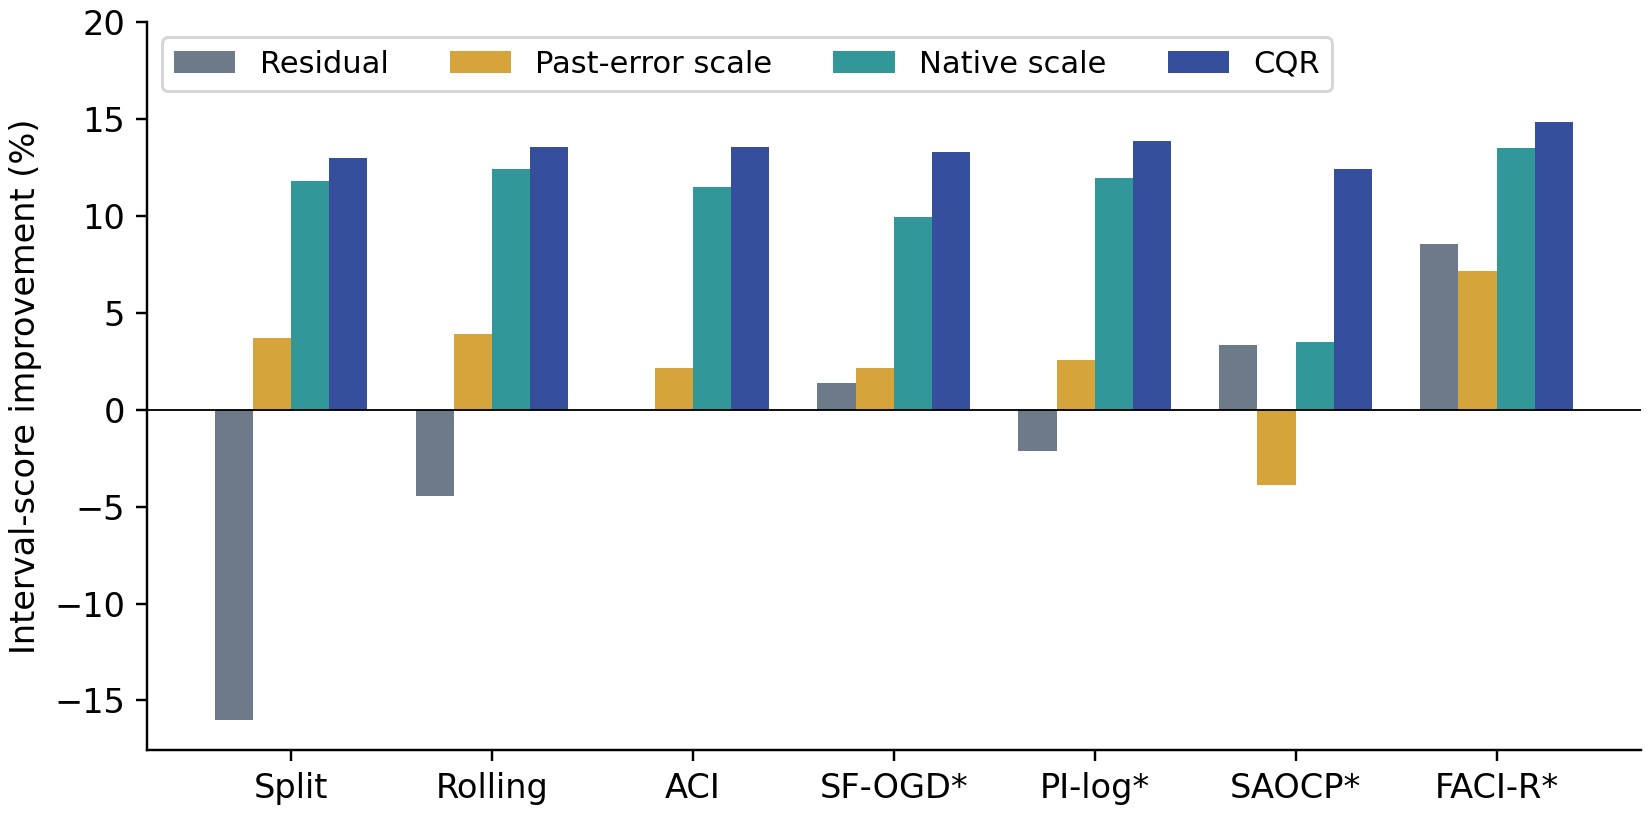
\includegraphics[width=\textwidth]{figures/score_rule.png}
\caption{Score--rule comparison on fixed one-step forecasts. Every gain uses the same
default residual--ACI denominator. Asterisks indicate the explicit adaptations described
in \ref{app:rules}; these labels do not claim equivalence to full original forecasting pipelines.}
\label{fig:rules}\end{figure}

\subsection{Benefits vary by family and persist on separate renewable series}
The mean CQR--ACI gain is 35.25\% on Alabama PV, 7.21\% on UCI loads, 5.96\% on ETT
and only 0.37\% on the three ERCOT loads (Table~\ref{tab:family}). The synthetic mean
is slightly negative. This heterogeneity is more informative than a pooled correlation
between a post-hoc volatility index and gains. Removing all eight PV series leaves
a 6.03\% gain, with descriptive interval $[4.25,7.88]\%$. Restricting to the 25 observed
series yields 15.16\%; that subset gives PV a larger relative weight. Leave-one-family-out
means remain positive, ranging from 6.03\% to 16.60\%.

\begin{table}[htbp]\centering\small
\caption{CQR--ACI gains by main-panel family. Intervals resample series within the listed
family and are descriptive; narrow intervals for correlated PV plants do not imply broad
geographic certainty. Small two- or three-series groups have especially limited precision.}
\label{tab:family}\begin{tabular}{lrrr}
\toprule
Family & Series & Gain (\%) & Descriptive 95\% CI \\
\midrule
Alabama PV & 8 & 35.25 & [34.75, 35.74] \\
Constructed seasons & 2 & 8.58 & [6.25, 10.90] \\
Constructed switches & 2 & 12.31 & [11.36, 13.27] \\
ERCOT & 3 & 0.37 & [-1.53, 1.86] \\
ETT & 4 & 5.96 & [3.41, 8.51] \\
Synthetic & 2 & -0.05 & [-0.42, 0.31] \\
UCI load & 10 & 7.21 & [5.53, 9.70] \\
\bottomrule
\end{tabular}
\end{table}
\begin{figure}[htbp]\centering
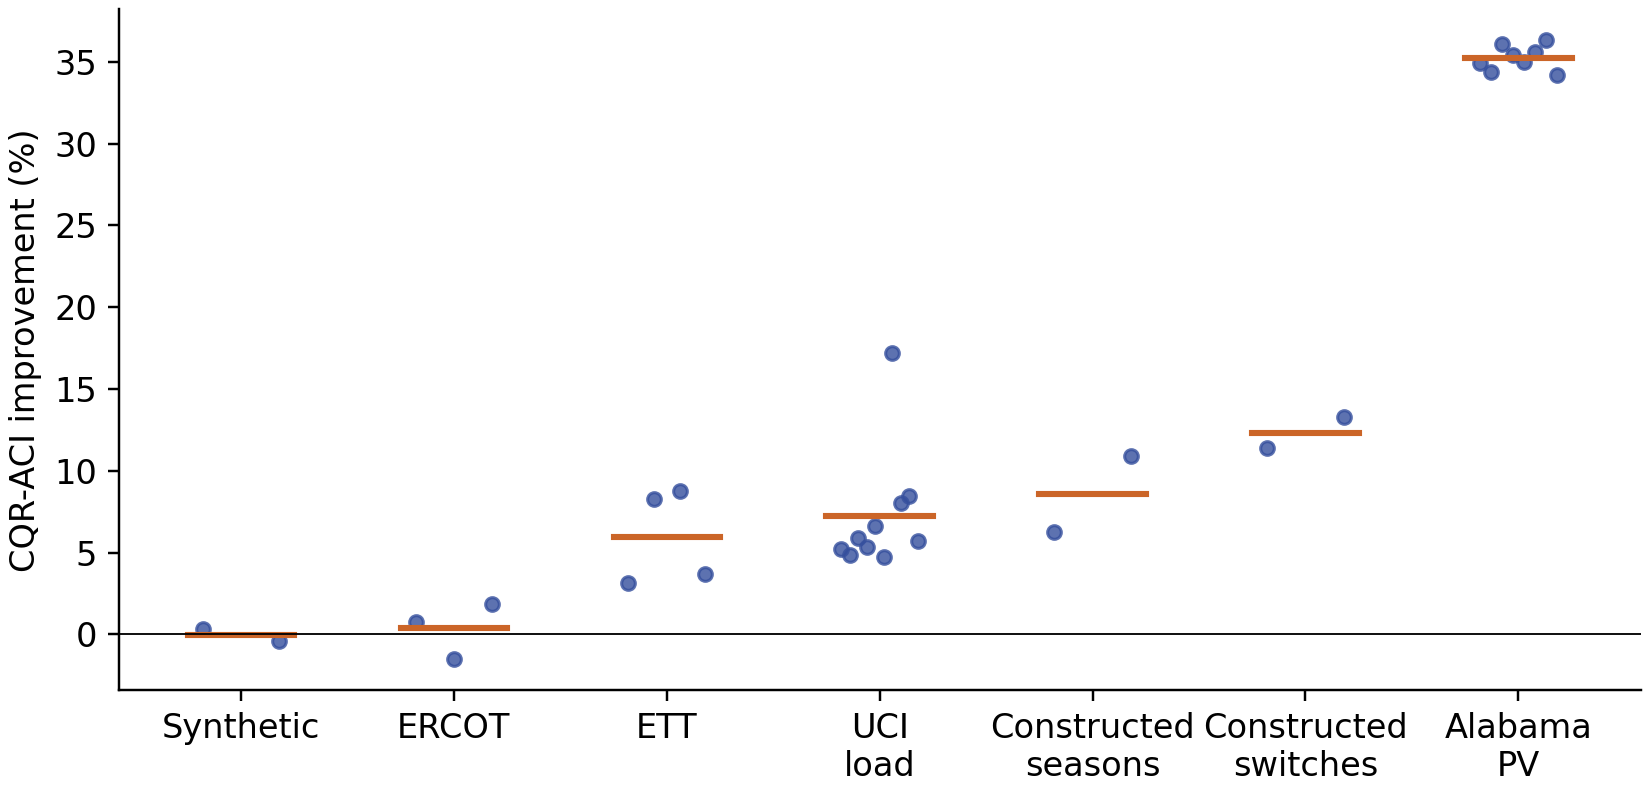
\includegraphics[width=\textwidth]{figures/families.png}
\caption{Each point is one series averaged across four backbones; horizontal orange marks
are family means. Constructed and synthetic series remain visible rather than being
counted as independent observed energy systems.}\label{fig:families}\end{figure}

Per-backbone mean gains are 15.15\% for Chronos-2, 13.82\% for Chronos-Bolt, 12.90\%
for Moirai and 12.41\% for the archived TimesFM configuration. On the separate GEFCom
panel, CQR--ACI gains 19.63\% overall: 41.46\% for solar and 13.08\% for wind, with
89.99\% mean coverage. This is evidence beyond the Alabama solar panel, but does not
convert correlated zones into independent geographic samples.

At block lengths 100, 200 and 400, 109 primary pairs have a positive paired-bootstrap
95\% interval and two have a negative interval. The centered-test/BH procedure identifies
109 positive and two negative differences at each of these block lengths. These counts
are reported with the dependence caveat above; the magnitude and family distribution of
the effect remain the main empirical evidence.

\subsection{Delayed feedback makes rule choice consequential}
Figure~\ref{fig:horizon} and Table~\ref{tab:horizon} show the joint horizon/feedback
experiment. At $h=24$, CQR--ACI has 87.34\% mean coverage, compared with 87.10\% for
residual--ACI. CQR--PI-log attains 89.96\% coverage and a 17.09\% score improvement
relative to residual--ACI, compared with 13.15\% for CQR--ACI. CQR--ACI's average number
of clipped updates, counting validation and test adaptation, increases from 3.06 at
$h=1$ to 201 at $h=24$. This is consistent with the projection term in
Equation~\eqref{eq:identity}, although a count alone does not measure its signed magnitude.

\begin{figure}[htbp]\centering
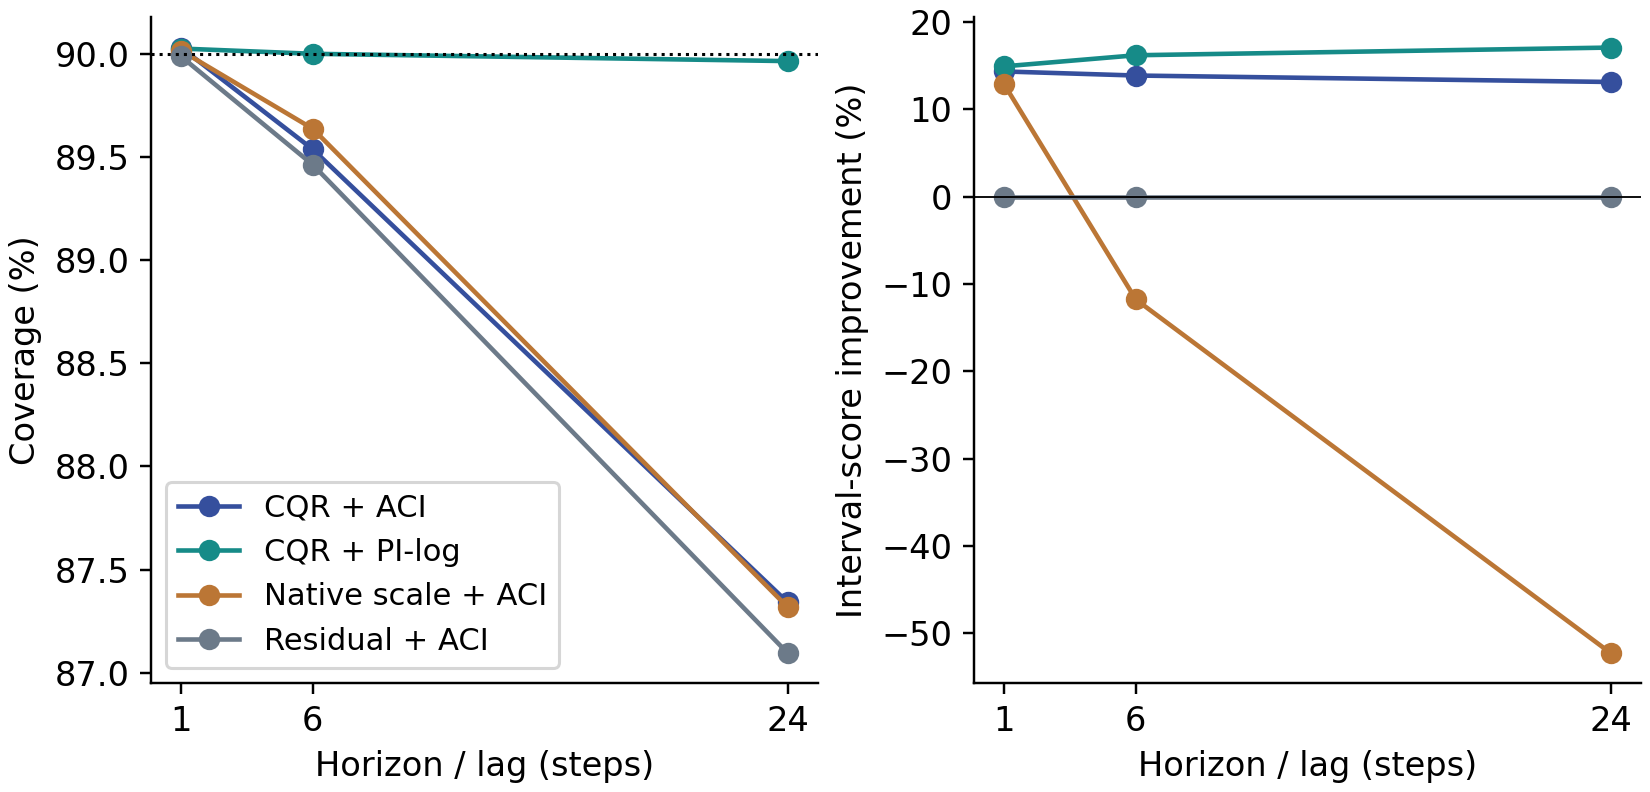
\includegraphics[width=\textwidth]{figures/horizon.png}
\caption{Joint changes in horizon and natural feedback delay on eight series and two
Chronos models. Coverage is an average; score gains use the horizon-specific residual--ACI
denominator. Solar steps are ten minutes, so $h=24$ is not day-ahead for those series.}
\label{fig:horizon}\end{figure}

The PI result is not a claim of uniformly improved reliability. At $h=24$, its local
150-origin coverage error is 4.86 percentage points, versus 4.52 for CQR--ACI. Improved
overall coverage can coexist with worse local variation. The controller also emits some
singletons after negative signed corrections: CQR--PI-log's average singleton rate is
0.567\% at $h=24$, versus 0.048\% for CQR--ACI. No infinite test intervals occur for
these two reported variants in this panel.

The fixed-forecast intervention separates lag from changing forecast difficulty
(Figure~\ref{fig:delay}). On the same $h=1$ predictions, increasing calibration lag from
1 to 24 steps changes residual--ACI coverage from 89.99\% to 88.62\% and CQR--ACI from
90.03\% to 89.52\%. CQR--PI-log remains at 89.99\% for lag 24, while its local coverage
error is 2.88 percentage points compared with 2.08 for CQR--ACI. Thus feedback restriction
alone can alter the relevant coverage comparison. The larger deficit in true $h=24$
forecasts additionally reflects changes in the forecast/score stream; lag alone does not
explain its entire magnitude.

\begin{figure}[htbp]\centering
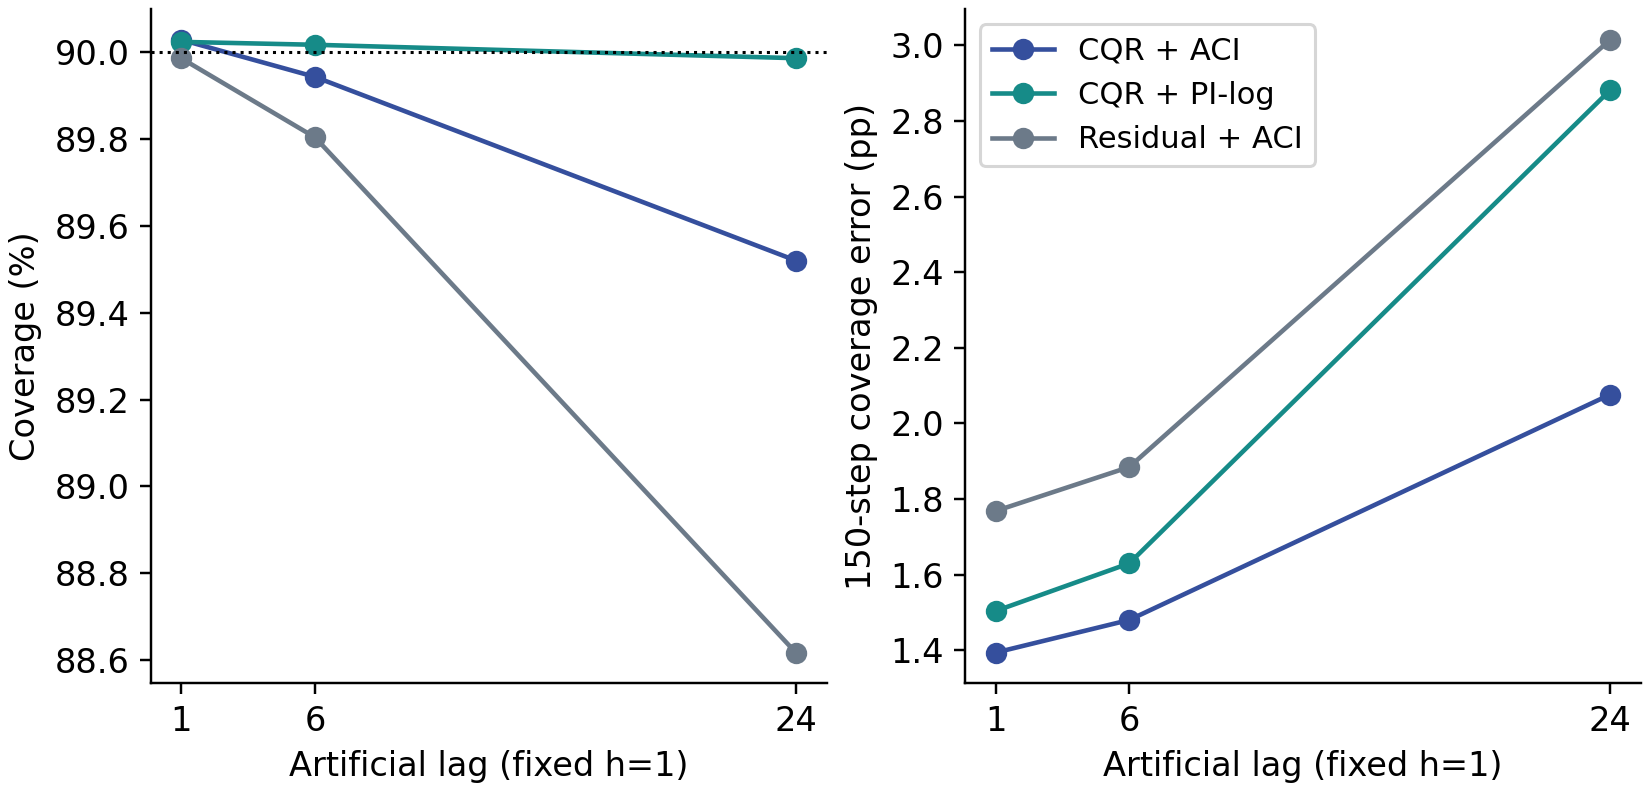
\includegraphics[width=\textwidth]{figures/delay_control.png}
\caption{Exploratory intervention holding one-step predictions and targets fixed while
withholding calibration outcomes. Overall coverage and local coverage error respond
differently. This isolates the calibrator's feedback channel, not the model's context.}
\label{fig:delay}\end{figure}

\subsection{Earlier long-horizon PV diagnostics}
The separate long-horizon diagnostic concerns two other development photovoltaic
series and two backbones, so it is not a within-panel comparison with the one-step
decomposition.
On the two development photovoltaic series and two backbones, tuned CQR--COP at
$h=24$ attains 90.41\% overall coverage, yet only 79.93\% on positive-output targets
and 97.05\% on zero-output targets (Figure~\ref{fig:solarconditional}). Zero outputs
constitute approximately 61.04\% of these test segments. At $h=1$ and $h=6$,
positive-output coverage is 87.95\% and 82.42\%, respectively, despite overall coverage
near 90\%. These are four model--series pairs from two series, not four independent
solar datasets. Positive output is an outcome-defined diagnostic and need not
coincide with astronomical daytime. A marginal coverage theorem does not promise
coverage on this subset, so the finding is not a counterexample to that theorem.

\begin{figure}[!htbp]\centering
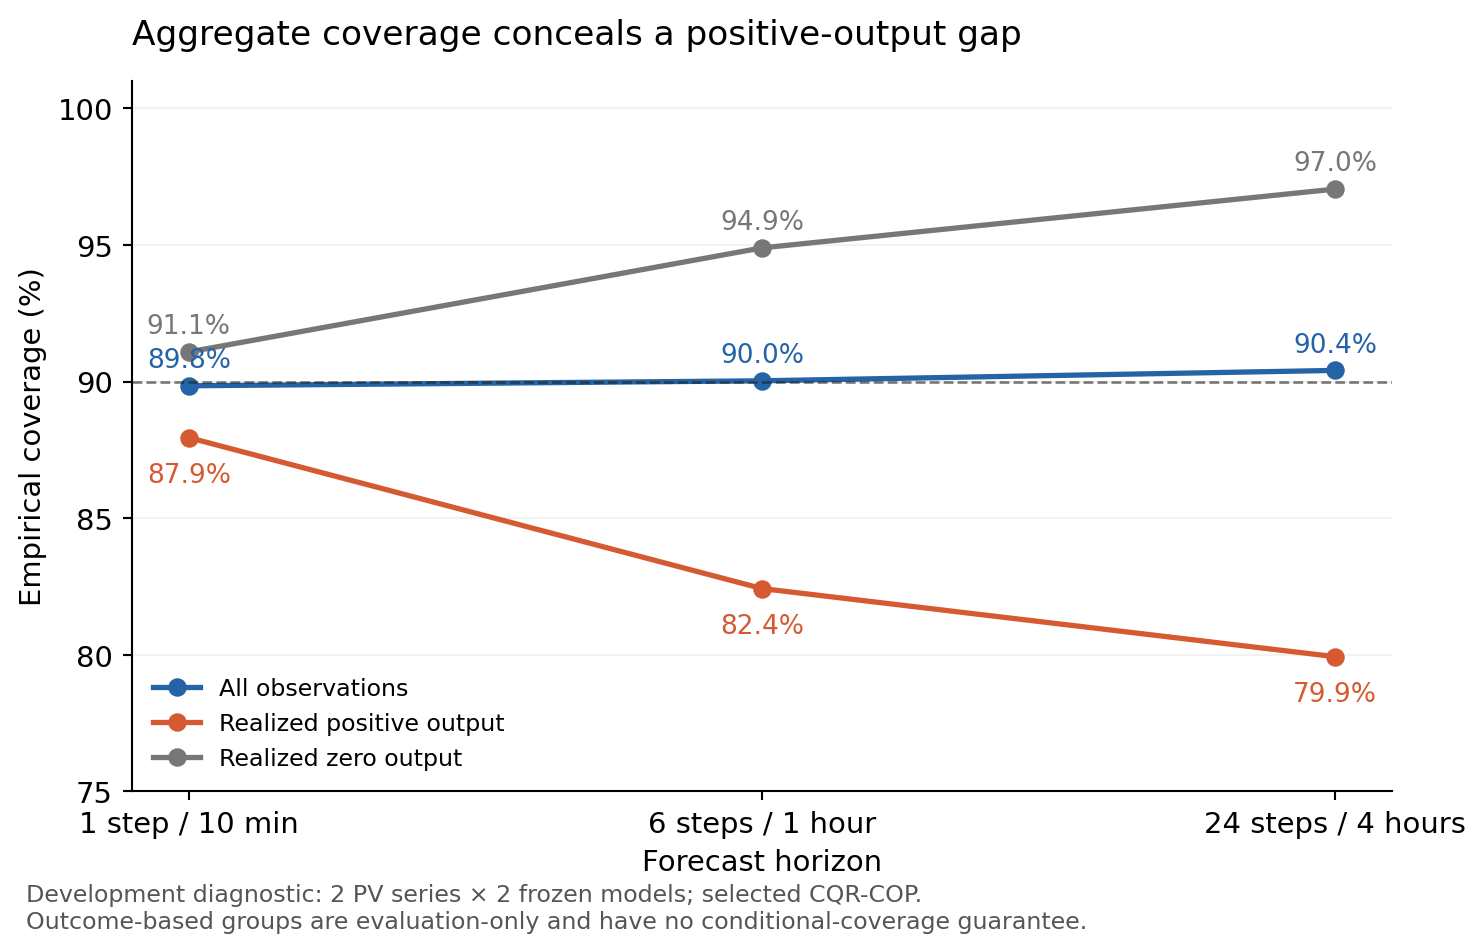
\includegraphics[width=\textwidth]{figures/solar_conditional_coverage.png}
\caption{Post-hoc photovoltaic reliability diagnostic for selected CQR--COP.
Coverages average over two series and two models. The zero/positive labels are used
only for evaluation; prediction and validation never use the future target label.
At this sampling rate, 24 steps represent four hours.}
\label{fig:solarconditional}\end{figure}

The observable-width grouping experiment tests whether a simple existing approach
can reduce the deficit. Separating both memory and state increases positive-output
coverage from 78.93\% to 83.49\% relative to matched shared-state CQR on these solar
pairs. Overall coverage changes from 88.46\% to 89.45\%, with a 2.47\% interval-score
gain. The positive-output gap remains substantial. Separating memory alone improves
solar interval score by 6.75\% but reduces overall coverage to 85.66\%, illustrating
why a proper-score change should be accompanied by coverage diagnostics.
Across all 16 development pairs, the both-grouped CQR gain is only 1.12\%.
On the confirmation families, the same grouping yields a 3.27\% gain at $h=24$,
but coverage remains 88.56\%, compared with 87.87\% for shared ACI. Grouping is thus
an informative control, not a demonstrated solution to conditional reliability.




\section{Detailed score constructions and original comparisons}\label{app:details}
\subsection{Scores and inversions}
Let $b_t=u_t-\ell_t$. We construct an outcome scale $v_t$ from a causal exponentially
weighted mean absolute error, updated only when a target is revealed, with decay 0.05.
Its initialization uses the first available forecast band and point prediction, not an
unseen outcome. The scale is bounded below by $10^{-12}$ for numerical arithmetic.
Define $\tilde b_t=\max(b_t,10^{-3}v_t)$. The four primary scores are
\begin{align}
 s_t^{\rm R}&=|y_t-m_t|,&
 s_t^{\rm E}&=|y_t-m_t|/v_t,\\
 s_t^{\rm N}&=|y_t-m_t|/\tilde b_t,&
 s_t^{\rm Q}&=\max(\ell_t-y_t,y_t-u_t).
\end{align}
They yield intervals $[m_t-q_t,m_t+q_t]$, $[m_t-v_tq_t,m_t+v_tq_t]$,
$[m_t-\tilde b_tq_t,m_t+\tilde b_tq_t]$ and $[\ell_t-q_t,u_t+q_t]$, respectively.
The native-scale control asks whether a native width helps without using native endpoints
directly; the past-error-scale control asks whether a simple outcome-based scale suffices.
CQR thresholds may be negative, allowing a band to shrink.

If inversion produces reversed endpoints, we record the event and emit a singleton at
their center. This is a practical interval repair rather than the exact empty set obtained
from signed-score inversion. Coverage-driven updates use the emitted interval. Infinite
intervals, if produced, are counted and retain infinite interval scores; they are not
capped or dropped. The primary CQR--ACI test intervals are singletons at an average rate
of 0.013\%, and no infinite intervals occur in the reported primary comparison.

We also examine normalized CQR, with denominator
$\max(b_t+\lambda v_t,10^{-3}v_t)$ for $\lambda\in\{0,0.01,0.1,0.5,1\}$.
A prefix selector chooses the lowest validation interval score among these five recipes
and the four primary scores under ACI. This is an existing model-selection principle used
as a diagnostic, not a proposed novel algorithm. A separate midpoint control replaces
$m_t$ by $(\ell_t+u_t)/2$ while retaining the residual or native-scale score.


\begin{table}[!htbp]\centering\small
\caption{Original one-step main-panel methods. Gain uses default residual--ACI;
Gap and Local denote absolute overall and 150-origin coverage errors in percentage points.}
\label{tab:main}\begin{tabular}{lrrrr}
\toprule
Score / rule & Gain (\%) & Cov. (\%) & Gap (pp) & Local (pp) \\
\midrule
residual/aci & 0.00 & 89.94 & 0.07 & 1.66 \\
error-scale/aci & 2.17 & 90.00 & 0.03 & 1.06 \\
native-scale/aci & 11.50 & 89.98 & 0.05 & 1.42 \\
cqr/aci & 13.57 & 89.98 & 0.05 & 1.45 \\
residual/faci & 8.57 & 89.19 & 0.81 & 1.86 \\
cqr/faci & 14.87 & 89.49 & 0.52 & 1.71 \\
residual/saocp & 3.32 & 92.54 & 2.64 & 2.92 \\
cqr/saocp & 12.40 & 90.73 & 1.49 & 2.07 \\
cqr/pi-log & 13.88 & 90.00 & 0.06 & 1.51 \\
cqr/sfogd & 13.28 & 90.00 & 0.03 & 0.98 \\
prefix-selected/aci & 13.72 & 89.98 & 0.05 & 1.46 \\
residual/aci/tuned & 5.23 & 89.74 & 0.28 & 1.65 \\
cqr/aci/tuned & 14.18 & 89.92 & 0.15 & 1.74 \\
\bottomrule
\end{tabular}\end{table}
\begin{table}[!htbp]\centering\scriptsize
\caption{Earlier CQR rate sensitivity at $h=24$. Development and traffic/exchange-rate
panels each have 16 pairs. S/I denote shared/issued. Selection uses validation only.}
\label{tab:rates}\begin{tabular}{llrrrrrr}
\toprule
Panel & Grid & Gain & Wins & Cov. S & Cov. I & Local S & Local I \\
\midrule
Development & original & 6.54 & 15/16 & 88.18 & 89.56 & 5.33 & 5.55 \\
Development & scaled & 0.73 & 13/16 & 89.54 & 89.35 & 5.62 & 5.60 \\
Development & wide & 0.59 & 13/16 & 89.45 & 89.32 & 5.66 & 5.61 \\
Traffic/FX & original & 8.43 & 16/16 & 87.87 & 89.43 & 5.79 & 6.12 \\
Traffic/FX & scaled & 1.27 & 13/16 & 89.00 & 89.03 & 6.14 & 6.25 \\
Traffic/FX & wide & 0.99 & 13/16 & 88.78 & 89.01 & 6.21 & 6.22 \\
\bottomrule
\end{tabular}
\end{table}
\begin{table}[!htbp]\centering\scriptsize
\caption{Original one-step PV decomposition. Contributions use each pair's overall
residual denominator and add to its overall gain; group gains use group denominators.}
\label{tab:solarparts}\begin{tabular}{llrrrrr}
\toprule
Settings & Group & Share & Gain & Contribution & Cov. R & Cov. CQR \\
\midrule
default & all & 100.00 & 35.25 & 35.25 & 89.88 & 89.96 \\
default & positive & 38.84 & 21.32 & 15.61 & 74.38 & 84.96 \\
default & zero & 61.16 & 73.37 & 19.64 & 99.72 & 93.14 \\
tuned & all & 100.00 & 20.51 & 20.51 & 89.34 & 89.72 \\
tuned & positive & 38.84 & 12.77 & 10.43 & 80.17 & 86.32 \\
tuned & zero & 61.16 & 54.89 & 10.08 & 95.16 & 91.88 \\
\bottomrule
\end{tabular}
\end{table}
\section{Detailed new-source protocol and reference comparison}\label{app:newprotocol}
\subsection{Protocol-locked confirmation on two new sources}\label{sec:newdesign}
After the preceding sensitivities, we fixed an additional protocol before numeric data
acquisition or calibration inspection. It selects MPI-BGC Jena roof temperature and
pressure for the first 3,600 hours of 2026, and PM2.5 at the Aotizhongxin and Dingling
stations for the first 3,600 hours from 1 March 2013 in the UCI Beijing archive
\citep{jena2026weather,chen2017air}. These are four series from two sources, evaluated
with the same two cached Chronos checkpoints: eight dependent model--series pairs.
Both models emit all 24 horizons at 2,976 consecutive origins. The main test segment
has 1,776 origins before excluding missing targets. Context length, batch size, dtype,
checkpoint-file hashes, timestamps and generation code are recorded for every archive.

Missing input observations are forward filled causally; missing targets are excluded
from score memory, controller increments and evaluation. Windows contain the latest
$W$ observed, revealed scores. Issued-state phases continue without an increment when
their outcome is missing. Local coverage uses 150 calendar-origin windows with their
observed denominators. The weather forecast targets are complete; the one missing
initial weather hour precedes all forecast contexts. The new-source protocol is locally
timestamped and hashed, not externally preregistered. Public historical air-quality data
may have been used in neural pretraining; new-to-calibration does not imply unseen-to-model.

For both scores and states, nested grids comprise the original rates at $W=450$;
the wide grid described below; and that grid augmented with zero
and four smaller rates ($10^{-6}$, $5\times10^{-6}$, $10^{-5}$ and $5\times10^{-5}$).
The final stage crosses these expanded rates with $W\in\{200,450,900\}$. Validation selects the minimum interval
score, breaking ties toward smaller rate and then window. Zero-rate trajectories
provide both fixed-window and selected-window rolling controls. Early and late
validation intervals, $[600+h-1,900-h+1)$ and $[900,1200-h+1)$, probe selector
stability without changing the primary full-validation selector or test segment.

The wide grid combines rates 0.0001, 0.0002, 0.0005, 0.001, 0.002, 0.005,
0.01, 0.02, 0.05 and 0.1 with the three original rates divided by $h$.

The predefined complete-weather subset also receives full AcMCP scorecasting: the
pinned author's MA$(h-1)$ plus cross-horizon regression implementation, at all horizons
1--24, with its supported CSS fitting option. We identify it as AcMCP-CSS, not the
default CSS-ML configuration. Rolling history is 600, $C_{\rm sat}=0.5$, and $K_I$
uses only the first 600 revealed target-clock error rows. The rate grid is
$\{0.001,0.005,0.01,0.05,0.1\}$ and these rates divided by $h$; the same validation
block selects it. Fitted scorecasts are independent of this rate, so they are cached
once per archive. A cached interval replay must agree with every original R trajectory
at rate 0.01 before evaluating the other rates. A matched no-scorecast PID control
uses the identical rate grid. Both are signed-error complete configurations; their
comparison to native CQR does not isolate controller quality.

\subsection{PV support and asymmetric-residual controls}\label{sec:pvcontrol}
On all 32 original one-step PV pairs, we additionally compare the established
signed-error construction
$[m_t+Q_{a_t/2}(Y-m),m_t+Q_{1-a_t/2}(Y-m)]$ with symmetric residuals and CQR.
It shares the total-miscoverage ACI state, timing and window. Each construction
uses the original nine rate/window settings; fixed defaults and a separately selected
zero-rate rolling control are retained. This is exploratory analysis of previously
inspected data, distinct from the new-source confirmation.

All three constructions are evaluated raw and after the same known-support projection
$[L,U]\mapsto[\max(0,L),\max(0,U)]$. Projected and raw configurations are separately
selected on validation score, while each candidate keeps its raw feedback trajectory:
the projection isolates interval geometry and is not a new feedback algorithm.
For a nonnegative target and finite ordered endpoints, projection cannot worsen
interval score or lose a covered target. In particular, when $L<0\leq U$, score
improvement is exactly $-L$, with unchanged coverage. When $U<0$, both endpoints
become zero and previously uncovered zeros can become covered. We therefore report
coverage changes as well as width and miss-distance penalties.

In addition to actual zero/positive targets, an observable grouping compares each point
forecast with the median of the first 600 point forecasts. This threshold is fixed
before validation; the high-forecast group is known at issue time and is not selected
using the future outcome. It is a diagnostic control, not a conditional-validity guarantee.

\begin{table}[!htbp]\centering\small
\caption{Original configured weather comparison using full validation. Ratios use
window-selected Rolling CQR; this precedes the common-history sensitivity.}
\label{tab:acmcpfull}\begin{tabular}{rlrrr}
\toprule
Horizon & Method & IS ratio & Coverage & Local \\
\midrule
1 & Rolling CQR & 1.000 & 89.37 & 3.15 \\
1 & Issued CQR & 0.996 & 89.44 & 1.43 \\
1 & AcMCP-CSS & 1.024 & 89.23 & 2.03 \\
1 & PID, no scorecast & 1.026 & 89.20 & 1.99 \\
6 & Rolling CQR & 1.000 & 90.27 & 2.91 \\
6 & Issued CQR & 1.002 & 90.44 & 2.91 \\
6 & AcMCP-CSS & 1.087 & 88.65 & 3.03 \\
6 & PID, no scorecast & 1.084 & 88.39 & 3.23 \\
24 & Rolling CQR & 1.000 & 89.51 & 6.03 \\
24 & Issued CQR & 1.000 & 89.43 & 6.01 \\
24 & AcMCP-CSS & 1.147 & 87.54 & 7.49 \\
24 & PID, no scorecast & 1.056 & 87.18 & 7.31 \\
\bottomrule
\end{tabular}
\end{table}
\section{Post-review temporal and history controls}\label{app:focused}
These analyses revisit inspected data. For positive-rate selectors, each state
minimizes the original full-validation score over the original stored positive
rates, then selects its window when allowed. The smallest rate is $10^{-6}$.
No candidate is added after test inspection. The air-quality CQR gaps are 0.0017\%
at $W=450$ and 0.0021\% with selected memory before admitting zero; these differences
are practically negligible. The paired records retain all rates and score scales.

Each test block contains 592 forecast origins. Missing labels are excluded using
the fixed observed mask. Local errors use 150-origin windows wholly within each
block, so whole-test local error is not exactly the weighted average of block values.
No configuration is reselected on a test block. Figure~\ref{fig:temporal} includes
every source, model and block; early/late validation sensitivity is a different analysis.
\begin{figure}[!htbp]\centering
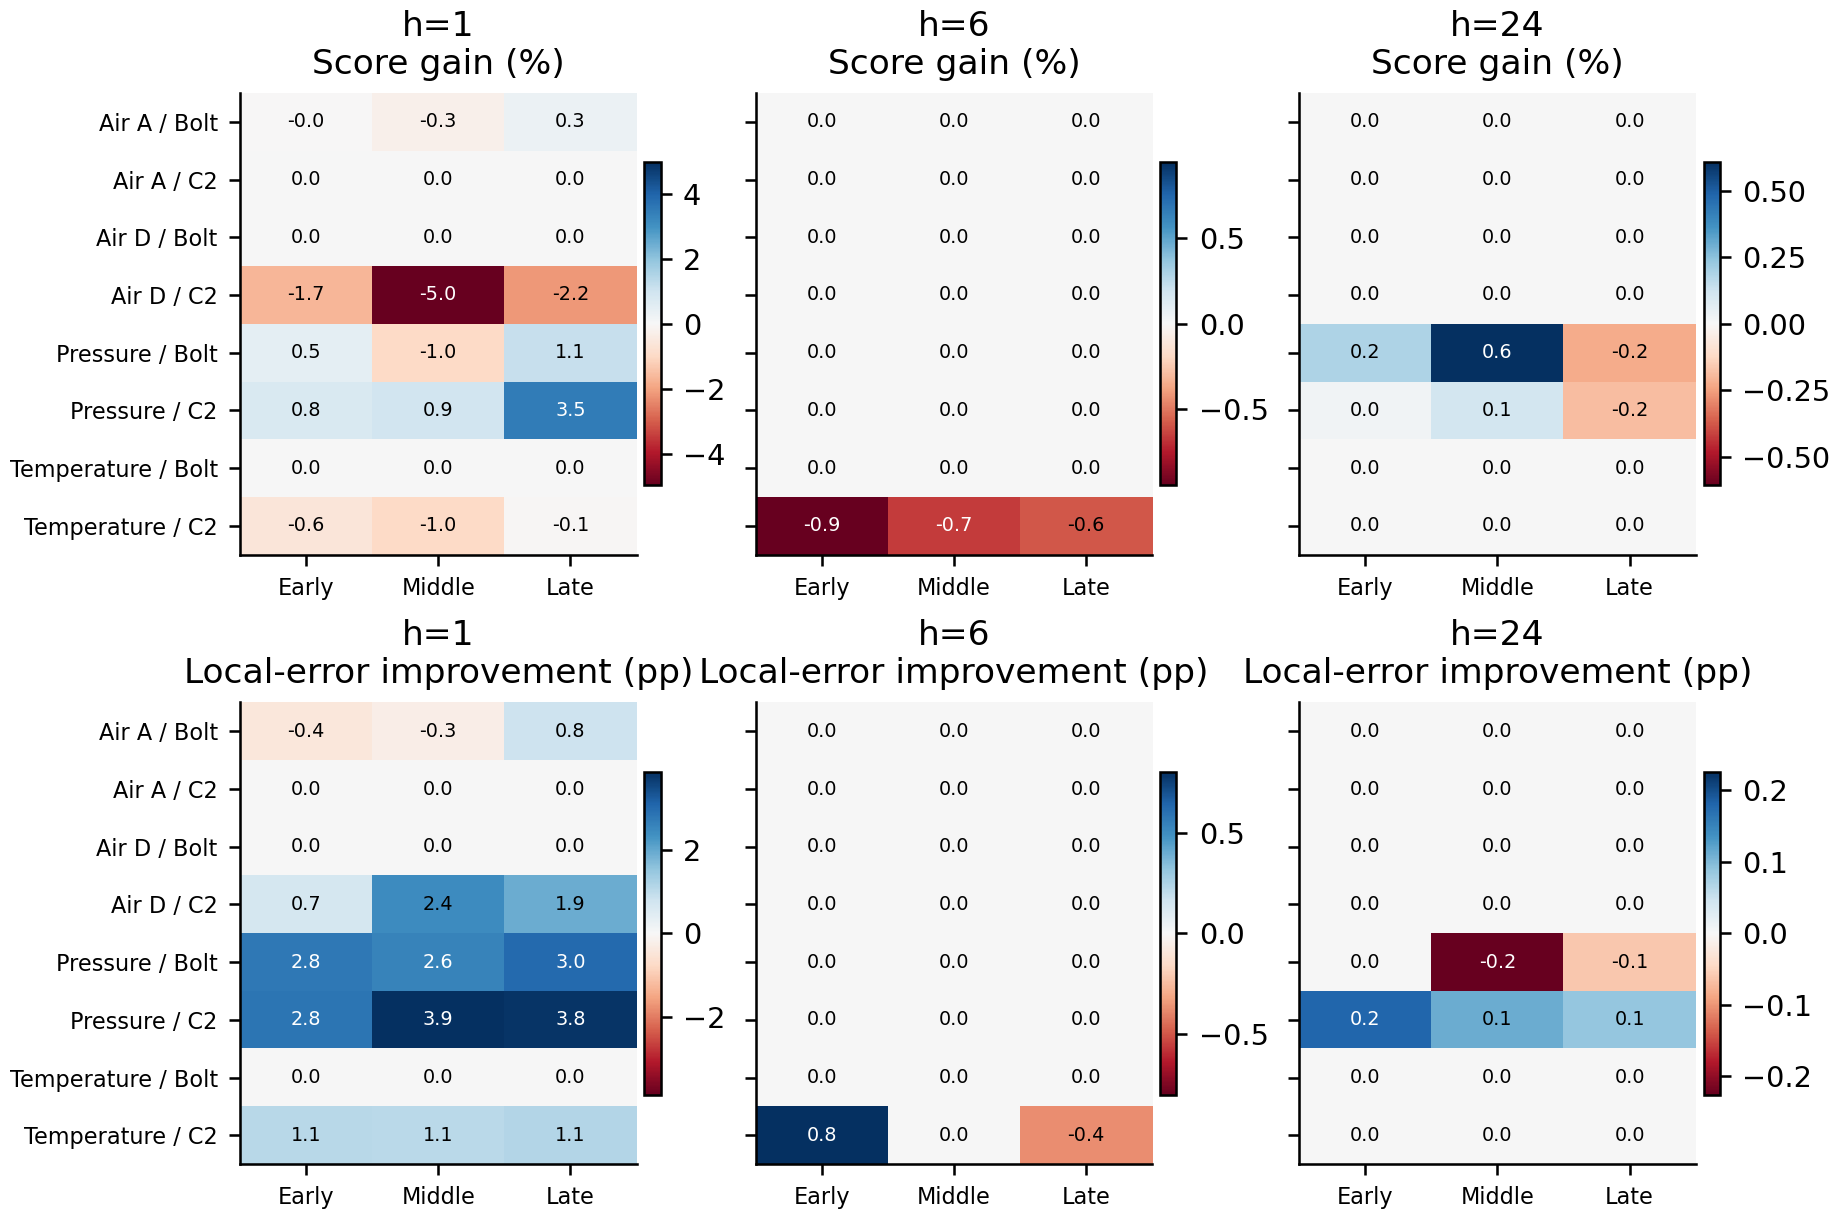
\includegraphics[width=\textwidth]{figures/temporal_pairs.png}
\caption{All eight new-source pairs, three consecutive test blocks. Positive means
issued CQR improves on matched selected-window Rolling CQR. Color scales differ
between panels; values are descriptive, without independent-replication error bars.}
\label{fig:temporal}\end{figure}

The common-history sensitivity adds unmodified author AcMCP-CSS at
$n_{\rm cal}=450$ to the saved $600$ runs. Both use $K_I$ from the first 600
revealed target-clock errors. Because history also changes startup, every method
uses post-startup validation $[900+h-1,1200-h+1)$ and unchanged testing
$[1200,2976)$. All evaluated scorecasts are finite. Each history selects its rate;
joint selection considers both histories. CQR retains its zero/small-rate grid;
PID uses AcMCP's rates with zero scorecasts. Each ratio uses its matched Rolling
denominator. History 900 and CSS-ML are outside this sensitivity.

All 60 sampled history-450 scorecast refits reproduce stored values. Three emit
an MA non-invertibility warning under CSS but return finite predictions. Their
warnings and trajectories are retained. These results characterize the stated
configuration, not default CSS-ML or every AcMCP setting.
\begin{table}[!htbp]\centering\scriptsize
\caption{Complete history sensitivity on all four weather pairs. IS ratios are
averaged after pairing. Coverage is percent and Local is percentage points.}
\begin{tabular}{rllrrr}
\toprule
Horizon & History & Method & IS ratio & Coverage & Local \\
\midrule
1 & 450 & Rolling-CQR & 1.000 & 89.64 & 3.32 \\
1 & 450 & CQR-shared & 0.993 & 89.68 & 1.63 \\
1 & 450 & CQR-issued & 0.993 & 89.68 & 1.63 \\
1 & 450 & AcMCP-CSS & 1.023 & 89.25 & 2.08 \\
1 & 450 & PID-no-scorecast & 1.024 & 89.32 & 1.86 \\
1 & 600 & Rolling-CQR & 1.000 & 89.64 & 3.44 \\
1 & 600 & CQR-shared & 0.995 & 89.60 & 1.71 \\
1 & 600 & CQR-issued & 0.995 & 89.60 & 1.71 \\
1 & 600 & AcMCP-CSS & 1.023 & 89.15 & 2.09 \\
1 & 600 & PID-no-scorecast & 1.024 & 89.32 & 1.86 \\
1 & 450/600 & Rolling-CQR & 1.000 & 89.58 & 3.40 \\
1 & 450/600 & CQR-shared & 0.994 & 89.58 & 1.72 \\
1 & 450/600 & CQR-issued & 0.994 & 89.58 & 1.72 \\
1 & 450/600 & AcMCP-CSS & 1.023 & 89.33 & 1.98 \\
1 & 450/600 & PID-no-scorecast & 1.024 & 89.32 & 1.87 \\
6 & 450 & Rolling-CQR & 1.000 & 89.74 & 2.91 \\
6 & 450 & CQR-shared & 1.018 & 89.96 & 2.45 \\
6 & 450 & CQR-issued & 1.004 & 89.85 & 2.97 \\
6 & 450 & AcMCP-CSS & 1.087 & 88.68 & 3.04 \\
6 & 450 & PID-no-scorecast & 1.087 & 88.84 & 2.97 \\
6 & 600 & Rolling-CQR & 1.000 & 89.95 & 2.83 \\
6 & 600 & CQR-shared & 1.014 & 90.15 & 2.58 \\
6 & 600 & CQR-issued & 1.008 & 90.06 & 2.68 \\
6 & 600 & AcMCP-CSS & 1.085 & 88.67 & 3.09 \\
6 & 600 & PID-no-scorecast & 1.091 & 88.94 & 2.97 \\
6 & 450/600 & Rolling-CQR & 1.000 & 89.96 & 2.86 \\
6 & 450/600 & CQR-shared & 1.029 & 90.09 & 2.24 \\
6 & 450/600 & CQR-issued & 1.004 & 90.20 & 2.79 \\
6 & 450/600 & AcMCP-CSS & 1.085 & 88.67 & 3.09 \\
6 & 450/600 & PID-no-scorecast & 1.091 & 88.94 & 2.97 \\
24 & 450 & Rolling-CQR & 1.000 & 89.32 & 6.33 \\
24 & 450 & CQR-shared & 1.136 & 83.22 & 8.96 \\
24 & 450 & CQR-issued & 1.000 & 89.27 & 6.34 \\
24 & 450 & AcMCP-CSS & 1.138 & 89.18 & 6.45 \\
24 & 450 & PID-no-scorecast & 1.061 & 88.20 & 6.49 \\
24 & 600 & Rolling-CQR & 1.000 & 89.44 & 6.75 \\
24 & 600 & CQR-shared & 1.039 & 87.43 & 7.42 \\
24 & 600 & CQR-issued & 1.000 & 89.43 & 6.74 \\
24 & 600 & AcMCP-CSS & 1.172 & 89.27 & 6.27 \\
24 & 600 & PID-no-scorecast & 1.067 & 88.37 & 6.43 \\
24 & 450/600 & Rolling-CQR & 1.000 & 89.44 & 6.75 \\
24 & 450/600 & CQR-shared & 1.039 & 87.43 & 7.42 \\
24 & 450/600 & CQR-issued & 1.000 & 89.43 & 6.74 \\
24 & 450/600 & AcMCP-CSS & 1.164 & 89.18 & 6.48 \\
24 & 450/600 & PID-no-scorecast & 1.065 & 88.60 & 6.24 \\
\bottomrule
\end{tabular}
\end{table}

